\newpage
\section{Versuchsaufbau}
\label{sec:Aufbau}

Zur Messung der Faraday-Rotation an verschiedenen GaAs-Halbleitern wird
der in Abbildung \ref{fig:Aufbau} dargestellte Versuchsaufbau verwendet.

\begin{figure}
  \centering
  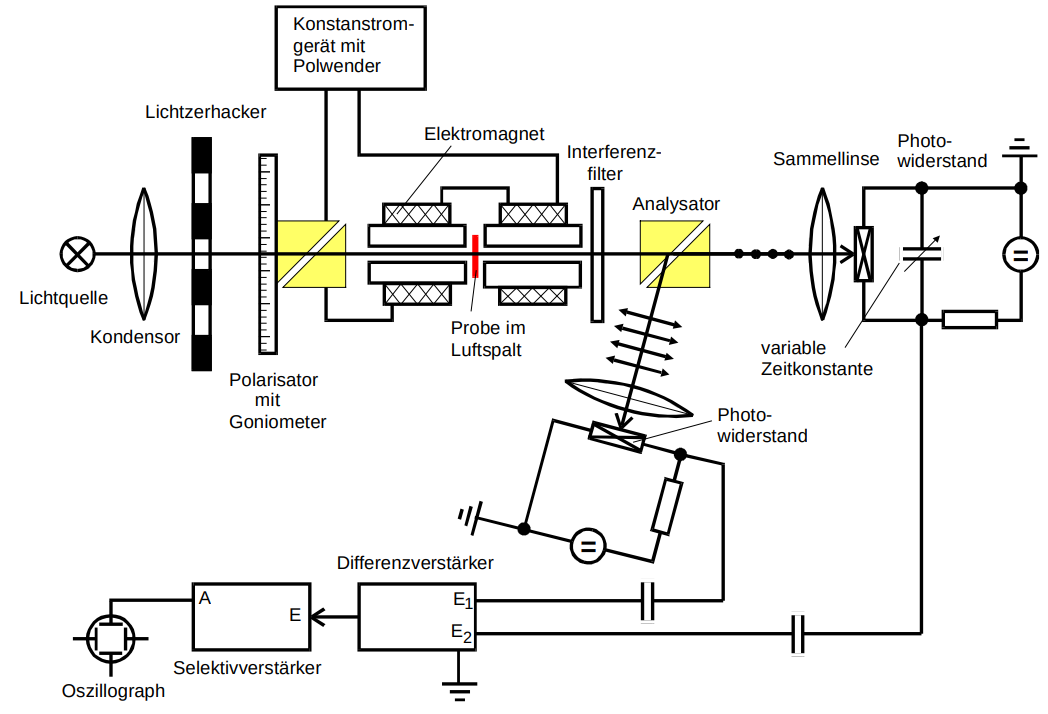
\includegraphics[width=\textwidth]{images/aufbau.pdf}
  \caption{Der verwendete Versuchsaubau schematisch dargestellt\cite[11]{anleitung}.}
  \label{fig:Aufbau}
\end{figure}

Das Licht einer Halogenlampe wird mit einem Kondensor (Sammellinse) parallelisiert
und mit einem Lichtzerhacker gepulst.
Die Amplitude des Lichtsignals oszilliert damit in der Frequenz des
Zerhackers. Im Anschluss fällt der Lichtstrahl auf ein Glan-Thomson
Prisma (Erläuterung weiter unten),
welches drehbar gelagert ist und das einfallende Licht linear polarisiert.
Der Drehwinkel dieses Polarisators ist an einem Goniometer ablesbar.
Das linear polarisierte Licht läuft durch einen Elektromagneten,
in welchem sich die zu untersuchende Probe in einem Luftspalt befindet.
Mit Hilfe eines Konstantstromgeräts kann somit ein externes Magnetfeld
an die Probe angelegt werden.

Hinter dem Elektromagneten wird das Licht mit Hilfe eines
Interferenzfilters monochromatisiert.
Ein Interferenzfilter besteht aus einem Dielektrikum zwischen zwei
transparenten Scheiben, in welchem die Lichtstrahlen an jeder
Schicht teilweise reflektiert werden. Insgesamt ergibt sich nur dann
eine Transmission, wenn diese Teilstrahlen konstruktiv interferieren.
Aufgrund der begrenzten Anzahl an reflektierenden Schichten ergibt sich
jedoch keine scharfe Spitze, sondern eine Verteilung endlicher Breite.
Das (nahezu) monochromatische Licht trifft auf ein zweites Glan-Thomson-Prisma,
welches den Lichtstrahl in zwei orthogonal zueinander
linear polarisierte Lichtstrahlen räumlich teilt.
Beide Strahlen werden jeweils mit einer Sammellinse auf einen
Photowiderstand fokussiert.

Die Photowiderstände befinden sich jeweils in einem geerdeten Schaltkreis
mit einer Spannungsquelle und einem Vorwiderstand.
Sie bestehen aus amorphen PbS Halbleitern.
% amorph: Keine Fernordnung, aber Nahordnung. => Unregelmäßige Muster
Je größer die Intensität des auf die Widerstände treffenden Lichtes ist,
desto mehr Elektronen werden
aus dem Halbleitermaterial heraus gelöst (äußerer Photoeffekt).
So entstehende Löcher werden mit Elektronen aus dem Schaltkreis gefüllt und
folglich fällt an dem Widerstand eine Spannung ab. Dieser Innenwiderstand
ist für viele Größenordnungen proportional zur Lichtintensität
\cite[11]{anleitung}.
An den Photowiderständen abfallende Wechselspannung wird auf Kondensatoren
ausgekoppelt, welche an einen Differenzverstärker angeschlossen sind.
Im Schaltkreis zur Messung des ordentlichen Strahlengangs
befindet sich parallel zum Photowiderstand geschaltet eine
regelbare Zeitkonstante. Sie ermöglicht eine Anpassung der
Phase an das Signal des anderen Photowiderstands.

Der Differenzverstärker bildet die Differenz der beiden
Wechselspannungen und gibt sie an
einen Selektivverstärker weiter.
Ein Selektivverstärker funktioniert ähnlich zu ein Bandpass mit regelbarer
Frequenz: Frequenzen, welche nicht der eingestellten Frequenz entsprechen,
werden gefiltert. Entscheidend ist dabei die Breite der Frequenzverteilung,
die durch die Güte $Q$ beschrieben wird.
Schließlich wird das gefilterte Signal auf einem Oszilloskop angezeigt.

\paragraph{Glan-Thomson-Prisma}
Ein Glan-Thomson-Prisma besteht aus einem doppelbrechendem Kristall,
der wie in Abbildung \ref{fig:GTP} dargestellt zerschnitten ist.
Linear polarisierte einfallende Strahlen werden in zwei senkrecht zueinander
linear polarisierte Strahlen aufgespalten.
Während der ordentliche Strahl an der Schnittfläche total refelktiert wird,
ändert der außerordentliche Strahl seine Ausbreitungsrichtung nicht.
\begin{figure}
  \centering
  \includegraphics[width=\textwidth]{images/gtp.pdf}
  \caption{Ein Glan-Thompson-Prisma schematisch dargestellt\cite[17]{anleitung}.}
  \label{fig:GTP}
\end{figure}

\section{Durchführung}
\label{sec:Durchführung}

\subsection{Messung der magnetischen Flussdichte der Spule}
\label{sec:MessungBFeld}

Das externe magnetische Feld, in welchem sich die Probe befindet, wird
mit Hilfe einer Hall-Sonde gemessen.
Dazu wird das Konstantstromgerät auf den für die spätere Messung verwendeten
maximalen Strom von ungefähr \SI{10}{\ampere} eingestellt und die
Spitze der Hall-Sonde mittig im Luftspalt positioniert.
In Abständen von \SI{1}{\milli\meter} wird nun die magnetische Flussdichte
in einem Bereich von \SI{10}{\milli\meter} jeweils vor und hinter der
Mitte des Luftspaltes vermessen.

\subsection{Kalibrierung des Aufbaus}
\label{sec:Kalibrierung}

Bevor die Faraday-Rotation vermessen werden kann, muss der Versuchsaufbau
justiert werden. Die Halogenlampe wird dazu mit einem
Konstantspannungsgerät bei ungefähr \SI{11}{\volt} betrieben und
Kondensor, Lichtzerhacker, Polarisator, Elektromagnet, Analysator und
die beiden Photowiderstände so aufgebaut, dass die beiden Lichtstrahlen auf
die Photowiderstände treffen.
Um diese Kalibrierung durch zu führen, werden die Deckel der
Photowiderstandsgehäuse entfernt.
Durch Verschiebung des Kondensors und der Sammellinsen in Strahlrichtung
kann die Lichtintensität auf den Photowiderständen maximiert werden.
Im Anschluss wird das Analysatorprisma um seine vertikale Achse so weit
gedreht, bis der durchgehende Strahl verschwindet.

Daraufhin wird der Lichtzerhacker auf eine Frequenz von ungefähr
\SI{590}{\hertz} eingestellt. Um die tatsächliche Frequenz zu ermitteln und
Fehler zu vermeiden, wird der Photowiderstand des durchgehenden
Strahles an das Oszilloskop angeschlossen und die Frequenz abgelesen.
Nun wird eine Probe in den Luftschaft des Elektromagneten gebracht und
die Photowiderstände an die Eingänge des Differenzverstärkers angeschlossen.
Dabei ist zu beachten, dass die Amplitude der jeweiligen
Wechselspannungen der Photowiderstände nicht \SI{100}{\milli\volt}
überschreitet. Angepasst wird dies durch Regelung der Intensität der
Halogenlampe über das Konstantspannungsgerät.
Ein Signal wird als \enquote{Ground}, das andere als Wechselstromsignal deklariert,
um ein möglichst klares Signal zu erhalten.

Der Ausgang des Differenzverstärkers wird mit dem Eingang des
Selektivverstärkers verbunden. Am Selektivverstärker wird die
Frequenz des Lichtzerhackers von \SI{590}{\hertz} sowie eine
maximal mögliche Güte von \num{100} eingestellt.
Schließlich wird der Ausgang des Selektivverstärkers an das Oszilloskop
angeschlossen. Durch Drehung des Polarisators und der Zeitkonstante
ist das Signal auf Null abzugleichen.


\subsection{Vermessung der Faraday-Rotation}
\label{sec:MessungFaraday}

Die Konstantstromquelle des Elektromagneten wird eingeschaltet und
langsam auf einen maximalen Strom von ungefähr \SI{10}{\ampere}
eingestellt. Nun werden für acht verschiedene Interferenzfilter
jeweils drei Proben in den Luftspalt eingesetzt und
das am Oszilloskop zu beobachtende Signal auf ein Minimum abgeglichen.
Hierzu wird die Zeitkonstante eines Photowiderstands angepasst und
der Polarisator gedreht. Mit Hilfe des Goniometers wird der Winkel
des Polarisators abgelesen und zusammen mit der Probe und dem verwendeten
Filter notiert.

Im Anschluss wird der Strom am Elektromagneten langsam auf \SI{0}{\ampere}
herunter gefahren, die Anschlüsse getauscht und wieder auf einen maximalen
Strom eingestellt. Wiederum werden die Proben für sämtliche Filter
eingesetzt, das Signal am Oszilloskop abgelesen und der Winkel des
Goniometers notiert.
Besonders bei dem Wechsel der Proben oder der Polarisationsfilter
ist darauf zu achten, dass die Amplitude der Wechselspannungen an den
Eingängen des Differenzverstärkers \SI{100}{\milli\volt} nicht
überschreitet.

Die verwendeten Proben sind
\begin{enumerate}
  \item n-dotiertes GaAs mit
  $N = \SI{2.8e18}{\raiseto{-3}\centi\meter}$ und
  $L = \SI{1.296}{\milli\meter}$
  \item n-dotiertes GaAs mit
  $N = \SI{1.2e18}{\raiseto{-3}\centi\meter}$ und
  $L = \SI{1.36}{\milli\meter}$
  \item hochreines GaAs mit
  $L = \SI{5.11}{\milli\meter}$
\end{enumerate}
Die Interferenzfilter sind für die Wellenlängen
\SIrange{1000}{1600}{\nano\meter} in \SI{1000}{\nano\meter}-Schritten
und zusätzlich \SI{1550}{\nano\meter} durchlässig.